% =====================================================================
%  Imaging Without Outcomes
%  Formatted for the AI for Meta-Science workshop, NeurIPS 2026
%
%  HOW TO BUILD THIS ON OVERLEAF
%  1. Download the official NeurIPS 2026 paper template zip from
%     https://neurips.cc/Conferences/2026/CallForPapers
%  2. Upload it to Overleaf as a new project. It contains neurips_2026.sty.
%  3. Replace the template's main .tex with THIS file, and upload the
%     figures/ folder alongside it.
%  4. Compile with pdfLaTeX.
%
%  BUILD MODES. One line, three outputs. Exactly one \usepackage line below
%  may be active.
%
%  [preprint]  ACTIVE, and the primary capstone artefact. Shows the author
%              block, no review line numbers, footnote names the target
%              venue without claiming submission or acceptance.
%
%  no option   Anonymised double blind build, for actually submitting to the
%              workshop. Suppresses the author block and adds line numbers.
%
%  [final,dblblindworkshop] plus \workshoptitle{AI for Meta-Science}
%              Camera ready, only appropriate if the paper is accepted. Do
%              not use it before then, since its footnote implies acceptance.
% =====================================================================

\documentclass{article}

\usepackage[preprint]{neurips_2026}
% \usepackage{neurips_2026}                            % anonymised submission
% \usepackage[final,dblblindworkshop]{neurips_2026}    % camera ready only

% Footnote text, set per build mode.
%
% The style file ships [dblblindworkshop] and \workshoptitle{}, but those set
% \@trackname, and \@trackname is only consulted inside \if@neuripsfinal. In
% preprint and submission modes the notice is hard coded, so it is overridden
% here. The guard leaves the camera ready build untouched, where the style
% file's own track name is correct.
\makeatletter
\if@neuripsfinal\else
  \if@preprint
    \renewcommand{\@noticestring}{%
      Preprint. Formatted for the AI for Meta-Science workshop (NeurIPS 2026).%
    }
  \else
    \renewcommand{\@noticestring}{%
      Submitted to AI for Meta-Science workshop (NeurIPS 2026). Do not distribute.%
    }
  \fi
\fi
\makeatother

\usepackage[utf8]{inputenc}
\usepackage[T1]{fontenc}
\usepackage{hyperref}
\usepackage{url}
\usepackage{booktabs}
\usepackage{amsfonts}
\usepackage{nicefrac}
\usepackage{microtype}
\usepackage{graphicx}
% Required. neurips_2026.sty defines the checklist answer macros as
% \textcolor{blue}{[Yes]}, \textcolor{orange}{[No]} and \textcolor{gray}{[N/A]}
% but does not load a colour package itself. Without this, \textcolor is
% undefined and its arguments are typeset as literal text. It must be xcolor
% rather than color, because gray and orange are not in the base colour set.
\usepackage{xcolor}

\title{Imaging Without Outcomes. A Targeted Rigor Appraisal of Medical
Imaging AI and the Limits of Automating It}

% Rendered in preprint and camera ready modes. The style file suppresses this
% block automatically in the anonymised submission build, so it is safe to
% leave populated. FILL IN the two lines marked below.
%
% DO NOT begin any of these lines with a square bracket. A line break followed
% by an open bracket is read as \\[<length>], the optional vertical space
% argument, so LaTeX tries to parse the text as a dimension, fails, and dumps
% the recovered characters into the page. If you ever do need a leading
% bracket here, write \\{}[like this] to shield it.
\author{%
  Adam T. Lane \\
  Your Institution Here \\
  \texttt{your.email@example.com} \\
}

\begin{document}

\maketitle

\begin{abstract}
Medical artificial intelligence tools are evaluated almost invariably on how well the model
discriminates. That is a claim about the model rather than a claim about the patient. We appraised
fifteen published imaging artificial intelligence papers against a thirteen item rigor checklist
drawn from standard clinical trial criteria, producing one hundred and ninety five justified
verdicts. Across the eleven paper primary set, external validation was satisfied by ten and a
genuine patient outcome was the primary endpoint of none, a paired difference of 90.9 percentage
points with an exact McNemar $p$ value of 0.0020 and no paper falling the other way. Transparent
reporting was also satisfied by no paper, so the evidentiary chain breaks at both ends rather than
one. We then asked whether the appraisal could be automated. A language model given only the written
rules and the papers reproduced the appraiser with a Cohen's kappa of 0.686, but its disagreements
concentrated in judging whether an item applied rather than in reading what a paper said. Rated
three times from cold it reproduced itself on 93.8 percent of cells where it had agreed with the
appraiser and 58.8 percent where it had not. Machine appraisal is least reliable exactly where it is
asked to do the most work.
\end{abstract}

\section{Introduction}
\label{sec:intro}

Meta-science asks what a literature actually establishes, as opposed to what it announces. That
question has become urgent in medical artificial intelligence, where the volume of published
evaluation now far exceeds the volume of evidence that any evaluated tool changed a patient's life.

The gap has a specific shape. Between a model's accuracy and a patient's benefit lies a chain of
evidence. A model is trained and reports internal accuracy. It is then validated on data it has not
seen. It is then evaluated prospectively. It is then, in principle, tested in a trial whose endpoint
is something that happens to a person rather than something that happens to a metric. Each link is
harder and more expensive than the one before it, and a paper may stop at any point and still be
publishable, useful and honest. This study asks where in that chain the published imaging
artificial intelligence literature actually stops.

We take imaging as the setting because it is where medical artificial intelligence is furthest
deployed. Autonomous diabetic retinopathy screening and computer aided polyp detection are
regulated, reimbursed and installed in clinics, so if any part of this literature had closed the
distance between discrimination and benefit, this is where the evidence should be.

The second question follows from the first, and it is the one that makes this a meta-science
problem rather than only a clinical one. Appraisal of this kind is slow. Fifteen papers read in
full, against thirteen items, with a written justification for every verdict, is a substantial
undertaking, and the reason appraisal of this kind does not scale is that it is bounded by expert
reading time. If a language model could reproduce such an appraisal from the written rules alone,
the bottleneck would move. So we ran that test directly and report what it does and does not
support.

Our contributions are as follows. First, a full rigor appraisal of the imaging artificial
intelligence literature, in which the evidentiary chain is shown to break at two points rather than
one, with the central comparison analysed as paired data. Second, a measurement of how far that
appraisal reproduces in the hands of an independent language model reader, together with a specific
and actionable account of where it fails, which is not where one would expect.

\section{The instrument}

The instrument is a thirteen item checklist assembled from criteria standard in the appraisal of
clinical trials and prognostic models.\footnote{The items reached this study as the appraisal
checklist taught in a graduate course on artificial intelligence in healthcare, which is the source
of the particular wording and ordering used here. The criteria themselves are long established and
none originates with that course or with this work. The attribution went unverified for part of the
study and was closed by checking every wording against the source, which found one item this project
had silently narrowed and reverted it before any analysis was finalised.} No item is original to this
work and the set is not offered as a novel instrument. Each item asks a single question with a Yes, No, Unclear or Not Applicable
answer, covering external validation, patient level randomised evaluation, prespecification of
endpoint and design, prospective registration, transparency of the model's predictors, honest
reporting of impact, independence from the maker of the tool, whether the primary endpoint is a
genuine patient outcome, sample size adequacy, intention to treat analysis, baseline comparability
and freedom from outcome leakage. The full wording of all thirteen is reproduced in Appendix
\ref{app:items}. The checklist was applied in its original form to a randomised trial of a
paediatric thromboembolism prognostic model \cite{walker2023}, which we retain here as an external
reference case.

What is specific to this study is not the items but a rule about when an item may be excused, and
that rule turns out to carry the whole design.

\paragraph{The item class rule.} Marking an item Not Applicable because a paper's design does not
reach it sounds fair. For the two items that measure clinical impact it is fatal. If only papers
that ran an impact trial are scored on whether they ran an impact trial, the denominator collapses
onto exactly the papers that pass, and the effect under measurement disappears by construction. We
therefore sorted items into four classes by what may excuse them. Items 2 and 9, which are the
dependent variables of the study, may never be excused. Items 3, 4, 5, 11 and 12 may be excused
only when a paper has no trial arms. Item 7 may be excused only when a paper contains no impact
evaluation at all. The remaining items are scored for every paper regardless of design. Not
Applicable is excluded from both numerator and denominator, so it never counts against a paper. The
classes are given in Appendix \ref{app:classes}.

\paragraph{Unclear as a verdict.} Unclear is a substantive verdict rather than a missing value.
Items 3 and 4 score Unclear when a trial is unregistered, because self reported prespecification
cannot be checked against anything. Item 5 scores Unclear when a trial was registered prospectively
but outside the register named in the item, which is not the same as reporting no registration.

\section{Corpus and procedure}
\label{sec:corpus}

Papers were identified through a prespecified PubMed search covering January 2018 to July 2026,
with the protocol frozen before the expansion search ran. Fifteen papers were appraised in full.
Eleven form the primary analysis set, four in retinal screening and seven in colonoscopy. Four
electrocardiography papers form a secondary set, reported separately and never pooled, because a
twelve lead electrocardiogram is a time series rather than an image. One further paper is the
reference case described above. Five further papers were screened, documented and deliberately not
scored, each with the exclusion criterion that placed it there. The corpus and the screening record
are given in Appendix \ref{app:corpus}, per item rates in Appendix \ref{app:items-rates}, per paper
scores in Appendix \ref{app:papers-scores}, and the secondary set and reference case in Appendix
\ref{app:secondary}.

Every paper was read in full and every verdict was assigned by hand with a written justification
quoting the passage that settles it, one paper at a time. An automated pass over the PDFs was used
to locate candidate evidence with page references, but it was never permitted to assign a verdict.
An earlier version of that tool offered suggested verdicts for the intention to treat item. Checked
against five papers it was wrong in five, by four distinct mechanisms, and the suggestion columns
were withdrawn.

Every interval reported in this paper is a two sided 95 percent confidence interval, abbreviated CI.
Single proportions carry Wilson score confidence intervals \cite{wilson1927,newcombe1998a}, with exact
Clopper-Pearson intervals \cite{clopper1934} computed alongside because several items sit at a
boundary. The central comparison is between two items scored on the same papers, so it is paired,
and it uses the Newcombe interval for paired proportions \cite{newcombe1998b} with an exact McNemar
test \cite{mcnemar1947}. Rates pooled over several items use a cluster bootstrap
\cite{efron1993} resampling papers rather than cells, since a paper contributes several correlated
cells. Choices between interval methods were fixed in advance rather than made once the numbers
were visible. Agreement is reported as Cohen's kappa \cite{cohen1960} alongside PABAK
\cite{byrt1993} and Gwet's AC1 \cite{gwet2008}, with Fleiss' kappa \cite{fleiss1971} for the three
pass self consistency measurement.

\section{Results}

\subsection{The chain breaks at both ends}

Table \ref{tab:groups} groups the thirteen items by the question they ask. The pattern is not a
gradient. It is two failures at opposite ends of the pipeline with competent work in between.

\begin{table}[t]
  \caption{Proportion of items satisfied across the eleven imaging papers, grouped by the question
  the items ask. Intervals are 95 percent confidence intervals.}
  \label{tab:groups}
  \centering
  \begin{tabular}{llrl}
    \toprule
    Item group & Items & Rate & 95 percent CI \\
    \midrule
    Model development, does the model work      & 1, 13             & 95.2 & 77.3 to 99.2 \\
    Trial conduct, was the study run properly   & 3, 4, 5, 10, 11, 12 & 72.4 & 54.0 to 89.6 \\
    Integrity, honest and independent reporting & 7, 8              & 55.0 & 31.6 to 77.3 \\
    Clinical impact, does it help patients      & 2, 9              & 36.4 & 19.7 to 57.0 \\
    \midrule
    Patient outcomes considered alone           & 9                 & 0.0  & 0.0 to 25.9 \\
    Transparency, is the model inspectable      & 6                 & 0.0  & 0.0 to 25.9 \\
    \bottomrule
  \end{tabular}
\end{table}

These papers reliably establish that the model works. They largely follow correct trial procedure.
They never establish that the model is inspectable, and they never establish that it helps
patients. Two of the thirteen columns contain no positive verdict at all, and both intervals run
from zero to 25.9, so neither excludes a true rate approaching one paper in four. The conclusion
survives at either end of both.

The refinement matters for how the result is stated. It would be convenient to say that model
development is the part that scores well. Transparency is also a model development property, and it
is one of the two worst performing columns in the appraisal.

\subsection{The narrowest comparison is the sharpest}

Table \ref{tab:contrast} reports the central contrast. External validation was satisfied by ten of
eleven papers. A genuine patient outcome was the primary endpoint in none. Because both items are
measured on the same eleven papers the comparison is paired, and every paper that differs falls the
same way.

\begin{table}[t]
  \caption{The primary paired contrast, external validation against patient outcomes, across the
  eleven imaging papers.}
  \label{tab:contrast}
  \centering
  \begin{tabular}{ll}
    \toprule
    External validation, item 1        & 10 of 11, 90.9 percent \\
    Genuine patient outcome, item 9    & 0 of 11, 0.0 percent \\
    Paired difference                  & 90.9 points, 95 percent CI 52.3 to 98.4 \\
    Test                               & exact McNemar, $p = 0.0020$, on 10 discordant papers \\
    Discordant the other way           & 0 papers \\
    \bottomrule
  \end{tabular}
\end{table}

At the group level the same claim holds. Ten of eleven papers score strictly higher on model
development than on clinical impact, one ties and none scores lower, giving a sign test $p$ of
0.0020. Figure \ref{fig:forest} shows every item ordered by rate.

\begin{figure}[t]
  \centering
  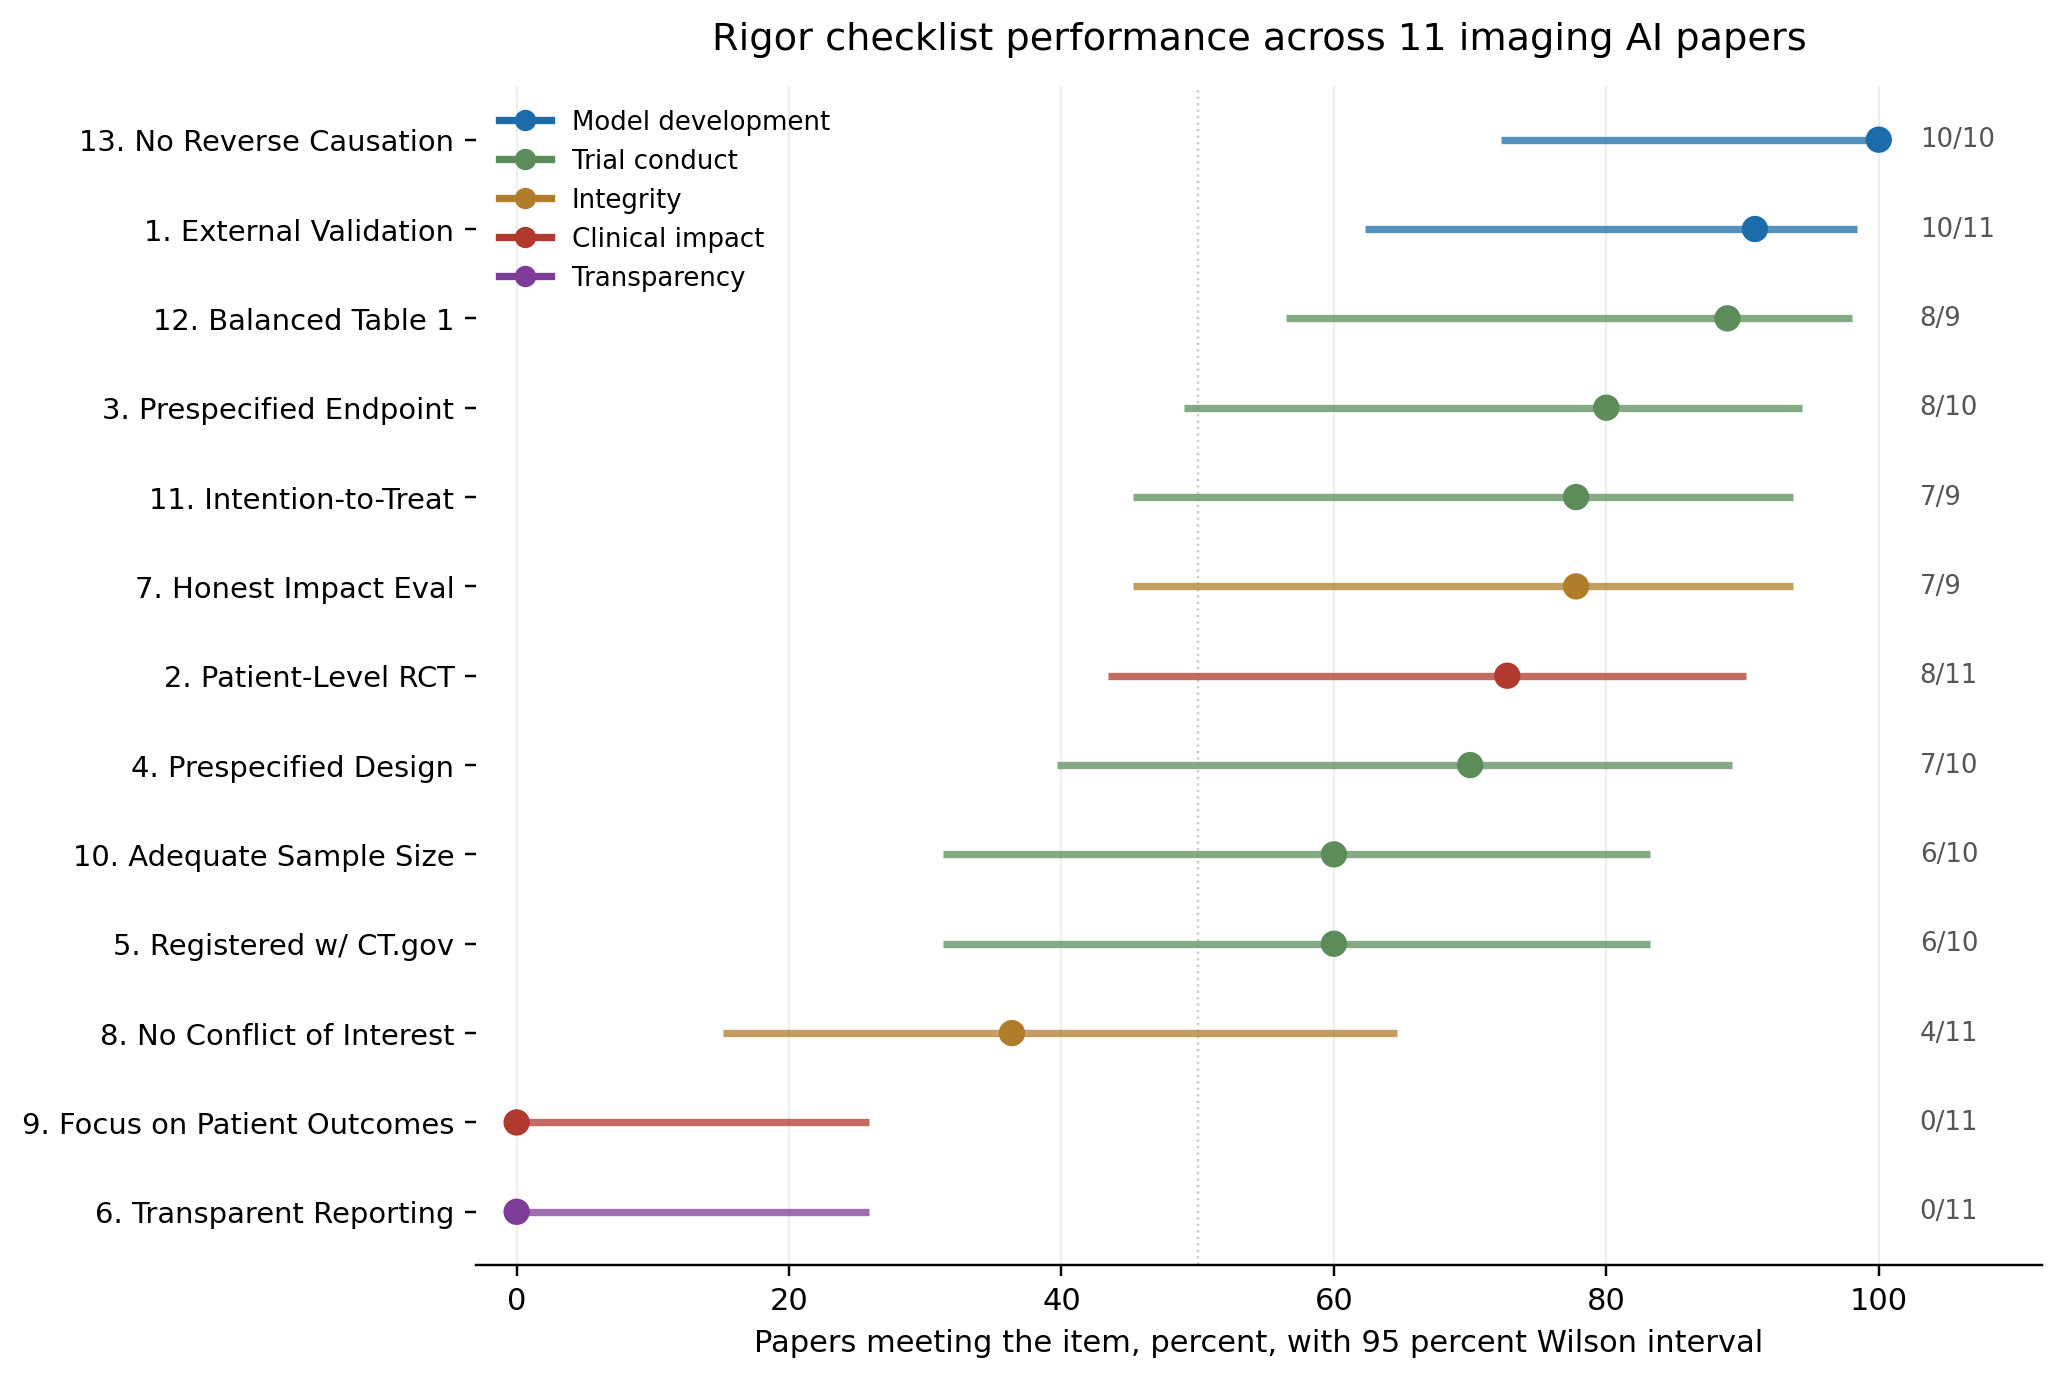
\includegraphics[width=0.92\linewidth]{figures/item_rates_forest.png}
  \caption{Proportion of papers satisfying each checklist item across the eleven imaging papers,
  ordered by rate, with 95 percent Wilson confidence intervals. The two items at zero, transparent reporting
  and patient outcomes, sit at opposite ends of the evidentiary chain.}
  \label{fig:forest}
\end{figure}

\subsection{Two findings we did not hypothesise}

\paragraph{Where these systems help, they help find what matters least.} Four of the colonoscopy
trials report gains concentrated in the lesions of least clinical consequence. Repici and colleagues
\cite{repici2020} found the entire gain in adenomas below ten millimetres with advanced adenoma
detection flat. Alali and colleagues \cite{alali2025} found the gain concentrated in diminutive
hyperplastic polyps. Wei and colleagues \cite{wei2023} and Hsu and colleagues \cite{hsu2026} found
more resections without more adenomas, and the latter quantified the cost, since computer aided
detection nearly doubled the proportion of patients assigned to intensive surveillance. The
checklist does not capture this pattern, which is a finding about the instrument as much as about
the papers.

\paragraph{Most of these trials were powered on baselines that reality contradicted.} Eight of the
eleven primary papers were randomised trials. Six of those eight built a power calculation on a
baseline event rate the observed data went on to contradict, which is 75.0 percent with a 95
percent confidence interval of 40.9 to 92.9. The reference case makes the same error in milder form, so the
problem is not specific to imaging.

\paragraph{Independence.} Four of eleven papers were clear of conflict of interest. Seven were
evaluated by people with a financial or ownership interest in the tool under test, or were funded
by its maker.

\section{Can the appraisal be automated}
\label{sec:auto}

No independent human second rater was available. A fallback had been specified in advance of any
second rating, and before any second rating result was seen, which fixed the order of preference
among possible raters and fixed what each could be called. Under it, a language model rating
supports a reproducibility check on the instrument and is never reported as inter rater
reliability. We report it in those terms here.

Five of the fifteen papers, sixty five cells, were rated independently by Gemini 3.6 Flash, a
language model from a developer other than the one whose assistant supported the first rater. The
selection was a seeded random draw stratified by domain, made before any second rating began,
because selecting the papers that appeared hardest would depress agreement by construction. The
rater received the
papers, the full item wordings, the item class rule, the Unclear conventions and a blank form. It
received no existing verdict, no justification note, no summary and no statement of what the study
predicted. Agreement was computed once from the independent ratings and was never recomputed.

\paragraph{What the first rating was, and why it bounds this result.} The appraiser is a single
person who read every paper in full and signed off on every verdict individually. That work was
itself assisted by a language model, which proposed each verdict together with a written
justification for the appraiser to accept, revise or reject before anything was recorded. Nothing
entered the record unreviewed, but the first pass over each item was not unaided.

Two things follow, and we would rather state them than leave a reader to discover them. This is why
the fallback protocol required the second rater to come from a different developer, since a rater
drawn from the same model family would be expected to share the first rater's blind spots rather
than expose them. It also bounds what the agreement figure can mean. The comparison is between a
model assisted appraisal carrying human sign off and an unassisted model reading, not between a
person and a machine, and the reproducibility claim should be read at that strength and no higher.

\begin{table}[t]
  \caption{Reproducibility of the appraisal by an independent language model reader working only
  from the written rules.}
  \label{tab:agree}
  \centering
  \begin{tabular}{lrr}
    \toprule
    & Substantive categories & Including Not Applicable \\
    \midrule
    Cells compared            & 47    & 65 \\
    Raw agreement             & 83.0 percent & 72.3 percent \\
    Cohen's kappa             & 0.686 & 0.591 \\
    PABAK                     & 0.745 & 0.631 \\
    Gwet's AC1                & 0.767 & 0.643 \\
    \bottomrule
  \end{tabular}
\end{table}

Table \ref{tab:agree} gives the result and Appendix \ref{app:agreement} breaks it down by item. A
kappa of 0.686 is substantial on the Landis and Koch convention \cite{landis1977}, and it supports
the statement that
the instrument is specified well enough that an independent reader working only from the written
rules reaches the same verdict in most cells. Three coefficients are reported together because the
verdicts are skewed toward Yes and no single coefficient is trustworthy under that skew.

\paragraph{The gap between the two columns is the finding.} Eighteen of the sixty five cells
disagree, and ten of the eighteen are disagreements about whether an item applied rather than about
what a paper reported. The instrument's substantive judgments reproduce considerably better than its
rules about applicability. The item class rule itself held in the sense that mattered most, since
neither rater placed Not Applicable on a class A item, which is the protection that stops the two
quantities the study measures from being excused on grounds of design.

\paragraph{Self consistency separates interpretation from noise.} The five papers were rated three
times, each pass in a fresh session with no memory of the others and with an identical prompt. This
is the one measurement a model rater supplies that a human cannot, since a person cannot be asked to
read a paper cold three times having forgotten the previous two. Agreement of the rater with itself
across the three passes gives a Fleiss' kappa of 0.844. Split by whether the first pass had agreed
with the appraiser, the rater reproduced itself on 93.8 percent of the cells where it agreed and on
58.8 percent of the cells where it disagreed. Its disagreements are concentrated where it is least
stable, so it is least reliable exactly where it is asked to do the most work.

\paragraph{Confidence carried no information.} The rater marked sixty four of sixty five cells as
high confidence and disagreed on twenty seven percent of those. Its single medium confidence cell
also disagreed. A human rater is asked to flag low confidence cells precisely because those are
where an instrument is doing least work. This rater produced none, and that is a real difference
between model and human rating rather than a detail of prompting.

\paragraph{What this licenses.} Two measurements that do not depend on one another point at the same
component. Ten of the eighteen disagreements concern applicability, and four of the ten cells the
rater could not reproduce for itself are the same kind of judgment. The least reproducible part of
this rigor instrument is its own rule about when an item applies. That is a finding about
instrument design, and it generalises beyond this checklist, because any appraisal instrument that
scales through automation will carry applicability rules of the same kind.

\section{Discussion}
\label{sec:discussion}

The clinical reading is that this literature is not dishonest. Several of the appraised papers are
explicit about precisely the limitation the appraisal records, and the most economical statement of
the problem comes from one of them. Ladabaum and colleagues \cite{ladabaum2023} introduced their
trial as a response to an expert consensus calling for studies of real world interaction between
clinicians and artificial intelligence that report relevant patient outcomes. They then reported
adenoma detection rates.
Even the study designed to close the outcomes gap measured detection instead. The failure is
structural. The field is measuring what it has collectively agreed to measure.

The meta-science reading is the one we want to press. Automating appraisal is attractive precisely
because appraisal is bounded by expert reading time, and our result is encouraging about the part
people worry about and discouraging about the part they do not. Extracting what a paper says is the
part that reproduces. Deciding whether a criterion applies to a given study design is the part that
does not, and it is also the part with the greatest capacity to change a headline number, because
applicability rules control denominators. An instrument whose applicability rules are loose can be
made to produce almost any rate without a single substantive verdict changing.

That suggests a concrete design principle for anyone building instruments intended to be applied at
scale by machine readers. Applicability should be specified at least as carefully as the criteria
themselves, and preferably reduced to a rule that depends on features of a study that can be read
off its design rather than judged. Our item class rule was written before scoring began and is
unusually explicit, and it still accounted for the majority of disagreements.

\section{Limitations}
\label{sec:limitations}

Eleven papers is a small sample. No item rate is pinned down to better than twenty six percentage
points and the median interval width across the thirteen items is forty five. The direction of the
central effect is established beyond reasonable doubt, because the comparison is paired and every
paper that differs falls the same way. The magnitude is not.

Only one database was searched. The protocol named two secondary databases to be used if the primary
returned too few eligible records in a domain. That condition was met in retinal imaging and the
secondary databases were nonetheless not searched. The protocol was also frozen partway through, so
ten of the fifteen papers were not selected under it. These two shortfalls are the reason this work
is presented as a targeted rigor appraisal rather than as a systematic review.

The reliability assessment was produced by a language model rather than an independent person, and
it does not meet, and is not offered as meeting, the standard that a human second rater would set.
It establishes that the written instrument reproduces in the hands of an independent reader. It
does not establish how two clinicians would differ. Neither side of that comparison is free of model
involvement, since the first rating was itself model assisted under human sign off, as section \ref{sec:auto}
records. It also rests on five papers and a single primary pass, and the model used was a fast tier
model, so the figures are better read as a floor than a ceiling.

Three items carry little information in this domain. One returned a single verdict across every
paper and is formally degenerate, because authors do not report their own data leakage and the
question cannot be answered from a published document. One item penalises a defensible design
choice, since cluster randomisation is arguably more rigorous for a tool that alerts a clinician
rather than treating a patient. Comparison between the two imaging domains cannot be supported at
this sample size and is reported as a demonstrated negative result rather than withdrawn.

One disclosure belongs here rather than in the acknowledgments, because it bounds how one result
should be read. The reference case is co authored by one of the two instructors who taught the
course from which this instrument derives, and it is the highest scoring document anywhere in the
collection at twelve of thirteen items, passing all four on which the imaging papers perform worst.
Neither instructor took any part in scoring it and neither was consulted on any verdict. Every
verdict on every paper was proposed and signed off by the author alone, one paper at a time, and the
reference case was scored on the same thirteen items on its own sheet and excluded from every
summary and export. It is also a single trial, so it anchors the comparison rather than testing it,
and no quantitative claim made here rests on it. The disclosure is made because an appraisal that
scores eleven other papers on undisclosed proximity between the evaluator and the evaluated should
be held to the rule it applies.

\section{Conclusion}

Across eleven imaging papers, two modalities, eight years and several countries, this literature
demonstrates repeatedly that its models discriminate well and never demonstrates that they are
inspectable or that they change what happens to patients. An independent language model reader
reproduces that appraisal well enough to be useful and fails in a specific and instructive place,
which is the judgment of whether a criterion applies at all. Appraisal instruments built to be read
by machines should be designed with that failure in mind.

\section*{Reproducibility statement}

An archive accompanies this paper containing all one hundred and ninety five verdicts with their
written justifications, the seven analysis notebooks, the fifteen derived data exports, the frozen
search protocol, the screening log, the full deviations log and the complete second rating record.
Every number in this paper regenerates from that archive.

The appraised papers themselves are not included, because they are published articles whose
copyright rests with their publishers. They are identified in full in the references and are
obtainable from those publishers, which is the ordinary arrangement for a review of published
literature. The
justification notes quote only the short passages that settle each verdict.

Deviations from the protocol are logged with dates and rationale, including two recorded late on
audit and one data handling error found and corrected during the study.

% The style file renders this as "Acknowledgments and Disclosure of Funding" and
% suppresses it automatically in the anonymised submission build, so it is safe
% to leave populated. It does not count against the page limit.
\begin{ack}
This work was carried out as a capstone project. The author thanks Dr. Ian McCulloh and Daniel
Byrne, MS, who taught the course in which it was undertaken, for the appraisal framework from which
the instrument used here is drawn and for guidance throughout.

Daniel Byrne is also a co author of the reference case. That relationship, and what it does and does
not bear on, is set out in Section \ref{sec:limitations}.

No funding was received for this work.
\end{ack}

\begin{thebibliography}{99}
\small

\bibitem{walker2023} Walker SC, French B, Moore RP, Domenico HJ, Wanderer JP, Mixon AS, Creech CB,
Byrne DW, Wheeler AP. Model-Guided Decision-Making for Thromboprophylaxis and Hospital-Acquired
Thromboembolic Events Among Hospitalized Children and Adolescents. The CLOT Randomized Clinical
Trial. \emph{JAMA Network Open}. 2023;6(10):e2337789.

\bibitem{zhou2023} Zhou Y, Chia MA, Wagner SK, et al. A foundation model for generalizable disease
detection from retinal images (RETFound). \emph{Nature}. 2023;622:156--163.

\bibitem{abramoff2018} Abramoff MD, Lavin PT, Birch M, Shah N, Folk JC. Pivotal trial of an
autonomous AI-based diagnostic system for detection of diabetic retinopathy in primary care offices
(IDx-DR). \emph{npj Digital Medicine}. 2018. doi 10.1038/s41746-018-0040-6.

\bibitem{wolf2024} Wolf RM, Channa R, Liu TYA, et al. Autonomous artificial intelligence increases
screening and follow-up for diabetic retinopathy in youth. The ACCESS randomized control trial.
\emph{Nature Communications}. 2024. doi 10.1038/s41467-023-44676-z.

\bibitem{mathenge2022} Mathenge W, Whitestone N, Nkurikiye J, et al. Impact of Artificial
Intelligence Assessment of Diabetic Retinopathy on Referral Service Uptake in a Low-Resource
Setting. The RAIDERS Randomized Trial. \emph{Ophthalmology Science}. 2022;2:100168.

\bibitem{repici2020} Repici A, Badalamenti M, Maselli R, et al. Efficacy of Real-Time
Computer-Aided Detection of Colorectal Neoplasia in a Randomized Trial. \emph{Gastroenterology}.
2020;159(2):512--520.

\bibitem{ahmad2023} Ahmad A, Wilson A, Haycock A, et al. Evaluation of a real-time computer-aided
polyp detection system during screening colonoscopy (AI-DETECT). \emph{Endoscopy}.
2023;55:313--319.

\bibitem{wei2023} Wei MT, Shankar U, Parvin R, et al. Evaluation of Computer-Aided Detection During
Colonoscopy in the Community (AI-SEE). \emph{American Journal of Gastroenterology}.
2023;118:1841--1847.

\bibitem{ladabaum2023} Ladabaum U, Shepard J, Weng Y, Desai M, Singer SJ, Mannalithara A.
Computer-aided detection of polyps does not improve colonoscopist performance in a pragmatic
implementation trial. \emph{Gastroenterology}. 2023. doi 10.1053/j.gastro.2022.12.004.

\bibitem{alali2025} Alali AA, Alhashmi A, Alotaibi N, Ali N, Alali M, Alfadhli A. Artificial
Intelligence for Adenoma and Polyp Detection During Screening and Surveillance Colonoscopy. A
Randomized-Controlled Trial. \emph{Journal of Clinical Medicine}. 2025;14:581.

\bibitem{kader2025} Kader R, Hassan C, Lanas A, et al. A novel cloud-based artificial intelligence
for real-time detection of colorectal neoplasia. A randomized controlled trial (EAGLE).
\emph{npj Digital Medicine}. 2025. doi 10.1038/s41746-025-02270-1.

\bibitem{hsu2026} Hsu WF, Kuo CY, Yen HH, et al. Computer-Assisted Colonoscopy in
High-Adenoma-Detection-Rate Settings in a High-Risk Population. A Randomized Clinical Trial.
\emph{JAMA Network Open}. 2026;9(4):e264881.

\bibitem{lin2024} Lin CS, Liu WT, Tsai DJ, et al. AI-enabled electrocardiography alert intervention
and all-cause mortality. A pragmatic randomized clinical trial. \emph{Nature Medicine}.
2024;30:1461--1470.

\bibitem{yao2021} Yao X, Rushlow DR, Inselman JW, et al. Artificial intelligence-enabled
electrocardiograms for identification of patients with low ejection fraction. A pragmatic,
randomized clinical trial (EAGLE). \emph{Nature Medicine}. 2021;27:815--819.

\bibitem{tsai2025} Tsai DJ, Lin C, Lee CC, et al. Artificial intelligence-assisted diagnosis and
prognostication in low ejection fraction using electrocardiograms in inpatient department. A
pragmatic randomized controlled trial. \emph{BMC Medicine}. 2025;23:342.

\bibitem{liu2025} Liu WT, Lin C, Lee CC, et al. Artificial Intelligence-Enabled ECGs for Atrial
Fibrillation Identification and Enhanced Outcomes (CARDIOLOGIST). \emph{Journal of the American
Heart Association}. 2025;14:e042106.

\bibitem{wilson1927} Wilson EB. Probable inference, the law of succession, and statistical
inference. \emph{Journal of the American Statistical Association}. 1927;22(158):209--212.

\bibitem{newcombe1998a} Newcombe RG. Two-sided confidence intervals for the single proportion.
Comparison of seven methods. \emph{Statistics in Medicine}. 1998;17(8):857--872.

\bibitem{clopper1934} Clopper CJ, Pearson ES. The use of confidence or fiducial limits illustrated
in the case of the binomial. \emph{Biometrika}. 1934;26(4):404--413.

\bibitem{newcombe1998b} Newcombe RG. Improved confidence intervals for the difference between
binomial proportions based on paired data. \emph{Statistics in Medicine}. 1998;17(22):2635--2650.

\bibitem{mcnemar1947} McNemar Q. Note on the sampling error of the difference between correlated
proportions or percentages. \emph{Psychometrika}. 1947;12(2):153--157.

\bibitem{efron1993} Efron B, Tibshirani RJ. \emph{An Introduction to the Bootstrap}. Chapman and
Hall. 1993.

\bibitem{cohen1960} Cohen J. A coefficient of agreement for nominal scales. \emph{Educational and
Psychological Measurement}. 1960;20(1):37--46.

\bibitem{landis1977} Landis JR, Koch GG. The measurement of observer agreement for categorical
data. \emph{Biometrics}. 1977;33(1):159--174.

\bibitem{byrt1993} Byrt T, Bishop J, Carlin JB. Bias, prevalence and kappa. \emph{Journal of
Clinical Epidemiology}. 1993;46(5):423--429.

\bibitem{gwet2008} Gwet KL. Computing inter-rater reliability and its variance in the presence of
high agreement. \emph{British Journal of Mathematical and Statistical Psychology}.
2008;61(1):29--48.

\bibitem{fleiss1971} Fleiss JL. Measuring nominal scale agreement among many raters.
\emph{Psychological Bulletin}. 1971;76(5):378--382.

\end{thebibliography}

\appendix

\section{The thirteen items}
\label{app:items}

Table \ref{tab:items} reproduces the instrument in the order in which it is applied. No item was
added, dropped or reordered during the study, and the wordings were frozen before the second rating
was run.

\begin{table}[h]
  \caption{The thirteen checklist items.}
  \label{tab:items}
  \centering
  \small
  \begin{tabular}{p{0.4cm}p{3.0cm}p{8.6cm}}
    \toprule
    \# & Short label & Item \\
    \midrule
    1  & External Validation      & The model has been shown to hold up on a separate external, temporal or geographic dataset, not just internal analysis. \\
    2  & Patient Level RCT        & There is a pragmatic, patient level randomised controlled trial of impact, usual care against usual care plus AI, not a provider selected or before and after comparison. \\
    3  & Prespecified Endpoint    & The primary endpoint was prespecified before the trial began. \\
    4  & Prespecified Design      & The study design was prespecified before the trial began. \\
    5  & Registered               & The trial was registered before initiation, with a registration number stated in the Methods. \\
    6  & Transparent Reporting    & The model's predictors and their relative importance are reported. The model is not a black box. \\
    7  & Honest Impact Eval       & The evaluation of the model's real world impact is rigorous and honestly reported, not overstated relative to the results. \\
    8  & No Conflict of Interest  & Clear of any conflict of interest. Operationalised as a conflict existing when an author or the study has a financial or ownership interest in the specific tool under evaluation, or when the tool's maker funded or sponsored the study. Equipment loan alone does not count. \\
    9  & Focus on Patient Outcomes & The endpoint is a genuine patient outcome such as mortality or major morbidity, not merely a process or surrogate measure such as a detection rate. \\
    10 & Adequate Sample Size     & The sample size is sufficiently large to detect the effect claimed, and not so large that trivial effects appear significant. \\
    11 & Intention to Treat       & The primary analysis follows the intention to treat principle. \\
    12 & Balanced Table 1         & The two study arms are shown to be comparable and balanced in a baseline table. \\
    13 & No Reverse Causation     & The model avoids reverse causation or data leakage, meaning an outcome used as a predictor. \\
    \bottomrule
  \end{tabular}
\end{table}

\section{The item class rule}
\label{app:classes}

\begin{table}[h]
  \caption{The item class rule governing when an item may be marked Not Applicable.}
  \label{tab:classes}
  \centering
  \small
  \begin{tabular}{llp{7.4cm}}
    \toprule
    Class & Items & Not Applicable permitted when \\
    \midrule
    A & 2, 9              & Never. These are the dependent variables of the study. \\
    B & 3, 4, 5, 11, 12   & The paper has no trial arms. \\
    C & 7                 & The paper contains no impact evaluation at all. \\
    D & 1, 6, 8, 10, 13   & Never. Scored for every paper regardless of design. \\
    \bottomrule
  \end{tabular}
\end{table}

Not Applicable is excluded from both numerator and denominator, so it never counts against a paper.
Eleven of the one hundred and ninety five verdicts are Not Applicable.

\section{The corpus}
\label{app:corpus}

Eighteen records were assessed and logged with an include or exclude decision and a reason. Fifteen
papers were appraised in full. Five further papers were documented and deliberately not scored,
each carrying the exclusion criterion that placed it there, and are retained in the archive rather
than deleted.

Two of the original twelve slots, which is seventeen percent, were found to contain a PDF that was
not the paper the manifest claimed. One held a pooled analysis in place of a trial and the other a
survey companion in place of its parent study. Both would have been caught by opening the file and
reading the first page. That check became a mandatory step, and on the first pass of eight new
downloads it rejected two more.

\begin{table}[h]
  \caption{The eleven papers in the primary analysis set.}
  \label{tab:corpus}
  \centering
  \small
  \begin{tabular}{llp{6.2cm}}
    \toprule
    Domain & Study & Design \\
    \midrule
    Retinal     & Zhou 2023, RETFound \cite{zhou2023}       & Foundation model development \\
    Retinal     & Abramoff 2018, IDx-DR \cite{abramoff2018} & Prospective diagnostic accuracy trial \\
    Retinal     & Wolf 2024, ACCESS \cite{wolf2024}         & Pragmatic randomised trial \\
    Retinal     & Mathenge 2022, RAIDERS \cite{mathenge2022} & Investigator masked randomised trial \\
    Colonoscopy & Repici 2020 \cite{repici2020}             & Randomised trial \\
    Colonoscopy & Ahmad 2023, AI-DETECT \cite{ahmad2023}    & Randomised trial \\
    Colonoscopy & Wei 2023, AI-SEE \cite{wei2023}           & Multicentre randomised trial \\
    Colonoscopy & Ladabaum 2023 \cite{ladabaum2023}         & Pragmatic implementation study \\
    Colonoscopy & Alali 2025 \cite{alali2025}               & Randomised trial \\
    Colonoscopy & Kader 2025, EAGLE \cite{kader2025}        & Pragmatic multicentre randomised trial \\
    Colonoscopy & Hsu 2026 \cite{hsu2026}                   & Multicentre open label randomised trial \\
    \bottomrule
  \end{tabular}
\end{table}

\section{Per item rates}
\label{app:items-rates}

\begin{table}[h]
  \caption{Proportion of papers satisfying each item in the primary analysis set, with 95 percent
  Wilson confidence intervals. Denominators differ because Not Applicable is excluded.}
  \label{tab:itemrates}
  \centering
  \small
  \begin{tabular}{llrrl}
    \toprule
    \# & Item & Met & Rate & 95 percent CI \\
    \midrule
    1  & External Validation       & 10 of 11 & 90.9 & 62.3 to 98.4 \\
    2  & Patient Level RCT         & 8 of 11  & 72.7 & 43.4 to 90.3 \\
    3  & Prespecified Endpoint     & 8 of 10  & 80.0 & 49.0 to 94.3 \\
    4  & Prespecified Design       & 7 of 10  & 70.0 & 39.7 to 89.2 \\
    5  & Registered                & 6 of 10  & 60.0 & 31.3 to 83.2 \\
    6  & Transparent Reporting     & 0 of 11  & 0.0  & 0.0 to 25.9 \\
    7  & Honest Impact Eval        & 7 of 9   & 77.8 & 45.3 to 93.7 \\
    8  & No Conflict of Interest   & 4 of 11  & 36.4 & 15.2 to 64.6 \\
    9  & Focus on Patient Outcomes & 0 of 11  & 0.0  & 0.0 to 25.9 \\
    10 & Adequate Sample Size      & 6 of 10  & 60.0 & 31.3 to 83.2 \\
    11 & Intention to Treat        & 7 of 9   & 77.8 & 45.3 to 93.7 \\
    12 & Balanced Table 1          & 8 of 9   & 88.9 & 56.5 to 98.0 \\
    13 & No Reverse Causation      & 10 of 10 & 100.0 & 72.2 to 100.0 \\
    \bottomrule
  \end{tabular}
\end{table}

\section{Per paper scores}
\label{app:papers-scores}

\begin{table}[h]
  \caption{Items satisfied by each paper in the primary analysis set. Denominators differ because
  papers without trial arms carry Not Applicable under the item class rule.}
  \label{tab:paperscores}
  \centering
  \small
  \begin{tabular}{lrr}
    \toprule
    Paper & Met & Rate \\
    \midrule
    Hsu 2026 \cite{hsu2026}              & 11 of 13 & 84.6 \\
    Wolf 2024, ACCESS \cite{wolf2024}    & 9 of 13  & 69.2 \\
    Repici 2020 \cite{repici2020}        & 9 of 13  & 69.2 \\
    Kader 2025, EAGLE \cite{kader2025}   & 9 of 13  & 69.2 \\
    Abramoff 2018, IDx-DR \cite{abramoff2018} & 7 of 11 & 63.6 \\
    Alali 2025 \cite{alali2025}          & 8 of 13  & 61.5 \\
    Mathenge 2022, RAIDERS \cite{mathenge2022} & 8 of 13 & 61.5 \\
    Ahmad 2023, AI-DETECT \cite{ahmad2023} & 7 of 13 & 53.8 \\
    Wei 2023, AI-SEE \cite{wei2023}      & 7 of 13  & 53.8 \\
    Zhou 2023, RETFound \cite{zhou2023}  & 2 of 5   & 40.0 \\
    Ladabaum 2023 \cite{ladabaum2023}    & 4 of 12  & 33.3 \\
    \bottomrule
  \end{tabular}
\end{table}

The lowest scoring paper is worth naming carefully. It reports a deliberately minimal real world
implementation study, and a design of that kind forfeits several checklist items at once. The score
reflects the checklist's fit to the design rather than the quality of the reporting, which is among
the most candid in the set.

\section{Secondary set and reference case}
\label{app:secondary}

The four electrocardiography papers are reported separately and never pooled with the primary set,
because a twelve lead electrocardiogram is a time series rather than an image. At four papers every
interval is too wide to support a claim and none is offered. The set is retained because it supplies
two things the primary set cannot.

The first is the only genuine patient outcome anywhere in the collection. Lin and colleagues
\cite{lin2024} took all cause mortality at ninety days as their primary endpoint and found it lower
with the alert, 3.6 against 4.3 percent. This is an illustrative positive case and no part of the
argument rests on it. The remaining two papers in the set are Yao and colleagues \cite{yao2021} and
Tsai and colleagues \cite{tsai2025}.

The second is the clearest demonstration that the outcome distinction is not pedantic. Liu and
colleagues \cite{liu2025} declared process measures as primary endpoints and genuine patient
outcomes as secondary ones. Two of four process endpoints improved, with anticoagulant prescribing
rising from 12.0 to 23.3 percent.
Not one patient outcome moved. Ischaemic stroke, cardiovascular death and all cause death were all
null. The same trial reports a clear positive on what the system did and a null on what happened to
the patients.

Conflict of interest is zero of four in this set and transparency is zero of four.

\begin{table}[h]
  \caption{The reference case compared against the primary analysis set on the four items where the
  primary set performs worst.}
  \label{tab:refcase}
  \centering
  \small
  \begin{tabular}{lll}
    \toprule
    Item & Primary set & Reference case \\
    \midrule
    2. Patient level randomised trial   & 8 of 11 & Met \\
    6. Transparent reporting            & 0 of 11 & Met \\
    9. Focus on patient outcomes        & 0 of 11 & Met \\
    8. Clear of any conflict of interest & 4 of 11 & Met \\
    \bottomrule
  \end{tabular}
\end{table}

The reference case satisfies twelve of thirteen items, higher than any appraised paper, and passes
all four items on which the primary set performs worst. It is a single trial, so it anchors the
comparison rather than testing it, and it must not be read as a statistical contrast.

It is instructive in one further way the checklist does not score. It satisfies almost every item
and still changed nothing, because the clinical teams declined to act on the model's recommendation
in roughly three quarters of eligible cases. A tool can pass every item on this checklist and still
fail the patient.

\section{Per item agreement}
\label{app:agreement}

\begin{table}[h]
  \caption{Per item agreement between the appraiser and the independent language model reader,
  across the five dual rated papers.}
  \label{tab:itemagree}
  \centering
  \small
  \begin{tabular}{lll}
    \toprule
    Item & Agreement & Note \\
    \midrule
    2 Patient Level RCT          & 5 of 5      & \\
    7 Honest Impact Eval         & 5 of 5      & \\
    9 Focus on Patient Outcomes  & 5 of 5      & carries the central finding \\
    6 Transparent Reporting      & 4 of 5      & \\
    13 No Reverse Causation      & 4 of 5      & \\
    1 External Validation        & 3 of 5      & most contested \\
    3, 4, 5, 8, 10, 11, 12       & 3 of 5 each & \\
    \bottomrule
  \end{tabular}
\end{table}

Item 9 reproduced completely. That item carries the central result of the study, so the claim that
these papers validate their models far more often than they measure patient outcomes is the claim
least exposed to rater subjectivity. Overall concordance on Not Applicable placement was 84.6
percent.

Two of the eighteen disagreements are artefacts of our own transcription rule rather than
differences of judgment. A quotation gate converts any verdict asserting the presence of something
to Unclear when no verbatim quotation supports it. Two cells rested instead on numeric evidence
drawn from a flow diagram and a baseline table, which is grounded in the paper but cannot be quoted
as prose. The rule was applied as written rather than amended a second time after its effects were
visible. Its cost runs in the conservative direction, depressing apparent agreement rather than
inflating it, so the reported figures are a floor.

% =====================================================================
%  NeurIPS Paper Checklist
%
%  Headings, questions and guidelines are byte identical to the official
%  checklist.tex from the NeurIPS 2026 template zip, verified 8 August
%  2026. The template states that questions must not be modified and that
%  the guidelines must be kept, so only the Answer and Justification lines
%  are ours. Do not hand edit the questions.
%
%  The template also requires the instruction block to be deleted while
%  keeping this section heading, and places the checklist after the
%  references and after any supplemental material, which is where it sits.
%  It does not count against the page limit.
% =====================================================================

\newpage
\section*{NeurIPS Paper Checklist}

\begin{enumerate}

\item {\bf Claims}
    \item[] Question: Do the main claims made in the abstract and introduction accurately reflect the paper's contributions and scope?
    \item[] Answer: \answerYes{}
    \item[] Justification: The abstract and Section \ref{sec:intro} claim two contributions, a rigor appraisal of the imaging artificial intelligence literature and a measurement of how far that appraisal reproduces under an independent language model reader. Both are delivered in Sections 4 and 5. Claims about magnitude are stated as bounded by interval width in Section \ref{sec:limitations}.
    \item[] Guidelines:
    \begin{itemize}
        \item The answer \answerNA{} means that the abstract and introduction do not include the claims made in the paper.
        \item The abstract and/or introduction should clearly state the claims made, including the contributions made in the paper and important assumptions and limitations. A \answerNo{} or \answerNA{} answer to this question will not be perceived well by the reviewers. 
        \item The claims made should match theoretical and experimental results, and reflect how much the results can be expected to generalize to other settings. 
        \item It is fine to include aspirational goals as motivation as long as it is clear that these goals are not attained by the paper. 
    \end{itemize}

\item {\bf Limitations}
    \item[] Question: Does the paper discuss the limitations of the work performed by the authors?
    \item[] Answer: \answerYes{}
    \item[] Justification: Section \ref{sec:limitations} is a dedicated limitations section. It records the sample size, the single database searched, the protocol frozen partway through the appraisal, the absence of a human second rater, the fact that neither side of the reliability comparison is free of model involvement, the withdrawal of the domain comparison, and the three items that carry little information in this domain.
    \item[] Guidelines:
    \begin{itemize}
        \item The answer \answerNA{} means that the paper has no limitation while the answer \answerNo{} means that the paper has limitations, but those are not discussed in the paper. 
        \item The authors are encouraged to create a separate ``Limitations'' section in their paper.
        \item The paper should point out any strong assumptions and how robust the results are to violations of these assumptions (e.g., independence assumptions, noiseless settings, model well-specification, asymptotic approximations only holding locally). The authors should reflect on how these assumptions might be violated in practice and what the implications would be.
        \item The authors should reflect on the scope of the claims made, e.g., if the approach was only tested on a few datasets or with a few runs. In general, empirical results often depend on implicit assumptions, which should be articulated.
        \item The authors should reflect on the factors that influence the performance of the approach. For example, a facial recognition algorithm may perform poorly when image resolution is low or images are taken in low lighting. Or a speech-to-text system might not be used reliably to provide closed captions for online lectures because it fails to handle technical jargon.
        \item The authors should discuss the computational efficiency of the proposed algorithms and how they scale with dataset size.
        \item If applicable, the authors should discuss possible limitations of their approach to address problems of privacy and fairness.
        \item While the authors might fear that complete honesty about limitations might be used by reviewers as grounds for rejection, a worse outcome might be that reviewers discover limitations that aren't acknowledged in the paper. The authors should use their best judgment and recognize that individual actions in favor of transparency play an important role in developing norms that preserve the integrity of the community. Reviewers will be specifically instructed to not penalize honesty concerning limitations.
    \end{itemize}

\item {\bf Theory assumptions and proofs}
    \item[] Question: For each theoretical result, does the paper provide the full set of assumptions and a complete (and correct) proof?
    \item[] Answer: \answerNA{}
    \item[] Justification: The paper contains no theoretical results.
    \item[] Guidelines:
    \begin{itemize}
        \item The answer \answerNA{} means that the paper does not include theoretical results. 
        \item All the theorems, formulas, and proofs in the paper should be numbered and cross-referenced.
        \item All assumptions should be clearly stated or referenced in the statement of any theorems.
        \item The proofs can either appear in the main paper or the supplemental material, but if they appear in the supplemental material, the authors are encouraged to provide a short proof sketch to provide intuition. 
        \item Inversely, any informal proof provided in the core of the paper should be complemented by formal proofs provided in appendix or supplemental material.
        \item Theorems and Lemmas that the proof relies upon should be properly referenced. 
    \end{itemize}

    \item {\bf Experimental result reproducibility}
    \item[] Question: Does the paper fully disclose all the information needed to reproduce the main experimental results of the paper to the extent that it affects the main claims and/or conclusions of the paper (regardless of whether the code and data are provided or not)?
    \item[] Answer: \answerYes{}
    \item[] Justification: The instrument is reproduced in full in Appendix A, the applicability rule in Appendix B and the corpus in Appendix C. The rating protocol, the random draw and its seed, the identity and version of the model rater and the number of passes are given in Section \ref{sec:auto}. The reproducibility statement describes the archive.
    \item[] Guidelines:
    \begin{itemize}
        \item The answer \answerNA{} means that the paper does not include experiments.
        \item If the paper includes experiments, a \answerNo{} answer to this question will not be perceived well by the reviewers: Making the paper reproducible is important, regardless of whether the code and data are provided or not.
        \item If the contribution is a dataset and\slash or model, the authors should describe the steps taken to make their results reproducible or verifiable. 
        \item Depending on the contribution, reproducibility can be accomplished in various ways. For example, if the contribution is a novel architecture, describing the architecture fully might suffice, or if the contribution is a specific model and empirical evaluation, it may be necessary to either make it possible for others to replicate the model with the same dataset, or provide access to the model. In general. releasing code and data is often one good way to accomplish this, but reproducibility can also be provided via detailed instructions for how to replicate the results, access to a hosted model (e.g., in the case of a large language model), releasing of a model checkpoint, or other means that are appropriate to the research performed.
        \item While NeurIPS does not require releasing code, the conference does require all submissions to provide some reasonable avenue for reproducibility, which may depend on the nature of the contribution. For example
        \begin{enumerate}
            \item If the contribution is primarily a new algorithm, the paper should make it clear how to reproduce that algorithm.
            \item If the contribution is primarily a new model architecture, the paper should describe the architecture clearly and fully.
            \item If the contribution is a new model (e.g., a large language model), then there should either be a way to access this model for reproducing the results or a way to reproduce the model (e.g., with an open-source dataset or instructions for how to construct the dataset).
            \item We recognize that reproducibility may be tricky in some cases, in which case authors are welcome to describe the particular way they provide for reproducibility. In the case of closed-source models, it may be that access to the model is limited in some way (e.g., to registered users), but it should be possible for other researchers to have some path to reproducing or verifying the results.
        \end{enumerate}
    \end{itemize}


\item {\bf Open access to data and code}
    \item[] Question: Does the paper provide open access to the data and code, with sufficient instructions to faithfully reproduce the main experimental results, as described in supplemental material?
    \item[] Answer: \answerYes{}
    \item[] Justification: An archive accompanies the paper containing all verdicts and justifications, the analysis notebooks, the derived exports, the frozen protocol and the second rating record. The appraised articles themselves cannot be redistributed because their copyright rests with their publishers, and they are identified in full in the references instead.
    \item[] Guidelines:
    \begin{itemize}
        \item The answer \answerNA{} means that paper does not include experiments requiring code.
        \item Please see the NeurIPS code and data submission guidelines (\url{https://neurips.cc/public/guides/CodeSubmissionPolicy}) for more details.
        \item While we encourage the release of code and data, we understand that this might not be possible, so \answerNo{} is an acceptable answer. Papers cannot be rejected simply for not including code, unless this is central to the contribution (e.g., for a new open-source benchmark).
        \item The instructions should contain the exact command and environment needed to run to reproduce the results. See the NeurIPS code and data submission guidelines (\url{https://neurips.cc/public/guides/CodeSubmissionPolicy}) for more details.
        \item The authors should provide instructions on data access and preparation, including how to access the raw data, preprocessed data, intermediate data, and generated data, etc.
        \item The authors should provide scripts to reproduce all experimental results for the new proposed method and baselines. If only a subset of experiments are reproducible, they should state which ones are omitted from the script and why.
        \item At submission time, to preserve anonymity, the authors should release anonymized versions (if applicable).
        \item Providing as much information as possible in supplemental material (appended to the paper) is recommended, but including URLs to data and code is permitted.
    \end{itemize}


\item {\bf Experimental setting/details}
    \item[] Question: Does the paper specify all the training and test details (e.g., data splits, hyperparameters, how they were chosen, type of optimizer) necessary to understand the results?
    \item[] Answer: \answerYes{}
    \item[] Justification: Section \ref{sec:corpus} gives the corpus, the scoring procedure and the statistical methods with the reason each was chosen over its obvious alternative. Section \ref{sec:auto} gives the second rating design, including what the rater received and what it was denied.
    \item[] Guidelines:
    \begin{itemize}
        \item The answer \answerNA{} means that the paper does not include experiments.
        \item The experimental setting should be presented in the core of the paper to a level of detail that is necessary to appreciate the results and make sense of them.
        \item The full details can be provided either with the code, in appendix, or as supplemental material.
    \end{itemize}

\item {\bf Experiment statistical significance}
    \item[] Question: Does the paper report error bars suitably and correctly defined or other appropriate information about the statistical significance of the experiments?
    \item[] Answer: \answerYes{}
    \item[] Justification: Every proportion carries a 95 percent Wilson confidence interval with exact Clopper-Pearson confidence intervals computed alongside, because several items sit at a boundary. The central contrast is analysed as paired data with a Newcombe interval and an exact McNemar test. Pooled rates use a cluster bootstrap over papers. Method choices were fixed before the numbers were visible.
    \item[] Guidelines:
    \begin{itemize}
        \item The answer \answerNA{} means that the paper does not include experiments.
        \item The authors should answer \answerYes{} if the results are accompanied by error bars, confidence intervals, or statistical significance tests, at least for the experiments that support the main claims of the paper.
        \item The factors of variability that the error bars are capturing should be clearly stated (for example, train/test split, initialization, random drawing of some parameter, or overall run with given experimental conditions).
        \item The method for calculating the error bars should be explained (closed form formula, call to a library function, bootstrap, etc.)
        \item The assumptions made should be given (e.g., Normally distributed errors).
        \item It should be clear whether the error bar is the standard deviation or the standard error of the mean.
        \item It is OK to report 1-sigma error bars, but one should state it. The authors should preferably report a 2-sigma error bar than state that they have a 96\% CI, if the hypothesis of Normality of errors is not verified.
        \item For asymmetric distributions, the authors should be careful not to show in tables or figures symmetric error bars that would yield results that are out of range (e.g., negative error rates).
        \item If error bars are reported in tables or plots, the authors should explain in the text how they were calculated and reference the corresponding figures or tables in the text.
    \end{itemize}

\item {\bf Experiments compute resources}
    \item[] Question: For each experiment, does the paper provide sufficient information on the computer resources (type of compute workers, memory, time of execution) needed to reproduce the experiments?
    \item[] Answer: \answerYes{}
    \item[] Justification: No model was trained. The entire analysis runs in minutes on a consumer laptop, and the second rating consisted of three sessions with a hosted language model.
    \item[] Guidelines:
    \begin{itemize}
        \item The answer \answerNA{} means that the paper does not include experiments.
        \item The paper should indicate the type of compute workers CPU or GPU, internal cluster, or cloud provider, including relevant memory and storage.
        \item The paper should provide the amount of compute required for each of the individual experimental runs as well as estimate the total compute. 
        \item The paper should disclose whether the full research project required more compute than the experiments reported in the paper (e.g., preliminary or failed experiments that didn't make it into the paper). 
    \end{itemize}
    
\item {\bf Code of ethics}
    \item[] Question: Does the research conducted in the paper conform, in every respect, with the NeurIPS Code of Ethics \url{https://neurips.cc/public/EthicsGuidelines}?
    \item[] Answer: \answerYes{}
    \item[] Justification: The study appraises published literature. It involves no human subjects, no personal data and no model release. Findings that weaken the authors' own hypothesis are reported rather than dropped, and errors made during the study are logged rather than concealed.
    \item[] Guidelines:
    \begin{itemize}
        \item The answer \answerNA{} means that the authors have not reviewed the NeurIPS Code of Ethics.
        \item If the authors answer \answerNo, they should explain the special circumstances that require a deviation from the Code of Ethics.
        \item The authors should make sure to preserve anonymity (e.g., if there is a special consideration due to laws or regulations in their jurisdiction).
    \end{itemize}


\item {\bf Broader impacts}
    \item[] Question: Does the paper discuss both potential positive societal impacts and negative societal impacts of the work performed?
    \item[] Answer: \answerYes{}
    \item[] Justification: Section \ref{sec:discussion} argues that automated appraisal fails specifically on applicability judgments, which control denominators and therefore headline rates. That is stated as a caution against deploying automated appraisal naively, alongside the positive case for scaling evaluation.
    \item[] Guidelines:
    \begin{itemize}
        \item The answer \answerNA{} means that there is no societal impact of the work performed.
        \item If the authors answer \answerNA{} or \answerNo, they should explain why their work has no societal impact or why the paper does not address societal impact.
        \item Examples of negative societal impacts include potential malicious or unintended uses (e.g., disinformation, generating fake profiles, surveillance), fairness considerations (e.g., deployment of technologies that could make decisions that unfairly impact specific groups), privacy considerations, and security considerations.
        \item The conference expects that many papers will be foundational research and not tied to particular applications, let alone deployments. However, if there is a direct path to any negative applications, the authors should point it out. For example, it is legitimate to point out that an improvement in the quality of generative models could be used to generate Deepfakes for disinformation. On the other hand, it is not needed to point out that a generic algorithm for optimizing neural networks could enable people to train models that generate Deepfakes faster.
        \item The authors should consider possible harms that could arise when the technology is being used as intended and functioning correctly, harms that could arise when the technology is being used as intended but gives incorrect results, and harms following from (intentional or unintentional) misuse of the technology.
        \item If there are negative societal impacts, the authors could also discuss possible mitigation strategies (e.g., gated release of models, providing defenses in addition to attacks, mechanisms for monitoring misuse, mechanisms to monitor how a system learns from feedback over time, improving the efficiency and accessibility of ML).
    \end{itemize}
    
\item {\bf Safeguards}
    \item[] Question: Does the paper describe safeguards that have been put in place for responsible release of data or models that have a high risk for misuse (e.g., pre-trained language models, image generators, or scraped datasets)?
    \item[] Answer: \answerNA{}
    \item[] Justification: No models, scraped datasets or generative artefacts are released. The archive contains appraisal verdicts and analysis code.
    \item[] Guidelines:
    \begin{itemize}
        \item The answer \answerNA{} means that the paper poses no such risks.
        \item Released models that have a high risk for misuse or dual-use should be released with necessary safeguards to allow for controlled use of the model, for example by requiring that users adhere to usage guidelines or restrictions to access the model or implementing safety filters. 
        \item Datasets that have been scraped from the Internet could pose safety risks. The authors should describe how they avoided releasing unsafe images.
        \item We recognize that providing effective safeguards is challenging, and many papers do not require this, but we encourage authors to take this into account and make a best faith effort.
    \end{itemize}

\item {\bf Licenses for existing assets}
    \item[] Question: Are the creators or original owners of assets (e.g., code, data, models), used in the paper, properly credited and are the license and terms of use explicitly mentioned and properly respected?
    \item[] Answer: \answerYes{}
    \item[] Justification: Every appraised paper is cited in full. The articles are not redistributed, and the justification notes quote only the short passages that settle each verdict.
    \item[] Guidelines:
    \begin{itemize}
        \item The answer \answerNA{} means that the paper does not use existing assets.
        \item The authors should cite the original paper that produced the code package or dataset.
        \item The authors should state which version of the asset is used and, if possible, include a URL.
        \item The name of the license (e.g., CC-BY 4.0) should be included for each asset.
        \item For scraped data from a particular source (e.g., website), the copyright and terms of service of that source should be provided.
        \item If assets are released, the license, copyright information, and terms of use in the package should be provided. For popular datasets, \url{paperswithcode.com/datasets} has curated licenses for some datasets. Their licensing guide can help determine the license of a dataset.
        \item For existing datasets that are re-packaged, both the original license and the license of the derived asset (if it has changed) should be provided.
        \item If this information is not available online, the authors are encouraged to reach out to the asset's creators.
    \end{itemize}

\item {\bf New assets}
    \item[] Question: Are new assets introduced in the paper well documented and is the documentation provided alongside the assets?
    \item[] Answer: \answerYes{}
    \item[] Justification: The appraisal record is the new asset. It is documented by the instrument in Appendix A, the applicability rule in Appendix B, and a written justification attached to each of the one hundred and ninety five verdicts.
    \item[] Guidelines:
    \begin{itemize}
        \item The answer \answerNA{} means that the paper does not release new assets.
        \item Researchers should communicate the details of the dataset\slash code\slash model as part of their submissions via structured templates. This includes details about training, license, limitations, etc. 
        \item The paper should discuss whether and how consent was obtained from people whose asset is used.
        \item At submission time, remember to anonymize your assets (if applicable). You can either create an anonymized URL or include an anonymized zip file.
    \end{itemize}

\item {\bf Crowdsourcing and research with human subjects}
    \item[] Question: For crowdsourcing experiments and research with human subjects, does the paper include the full text of instructions given to participants and screenshots, if applicable, as well as details about compensation (if any)? 
    \item[] Answer: \answerNA{}
    \item[] Justification: The study involves no human participants. The only rater besides the author was a language model, and what it was given and denied is described in Section \ref{sec:auto}.
    \item[] Guidelines:
    \begin{itemize}
        \item The answer \answerNA{} means that the paper does not involve crowdsourcing nor research with human subjects.
        \item Including this information in the supplemental material is fine, but if the main contribution of the paper involves human subjects, then as much detail as possible should be included in the main paper. 
        \item According to the NeurIPS Code of Ethics, workers involved in data collection, curation, or other labor should be paid at least the minimum wage in the country of the data collector. 
    \end{itemize}

\item {\bf Institutional review board (IRB) approvals or equivalent for research with human subjects}
    \item[] Question: Does the paper describe potential risks incurred by study participants, whether such risks were disclosed to the subjects, and whether Institutional Review Board (IRB) approvals (or an equivalent approval/review based on the requirements of your country or institution) were obtained?
    \item[] Answer: \answerNA{}
    \item[] Justification: No human subjects research was conducted. The unit of analysis is a published paper.
    \item[] Guidelines:
    \begin{itemize}
        \item The answer \answerNA{} means that the paper does not involve crowdsourcing nor research with human subjects.
        \item Depending on the country in which research is conducted, IRB approval (or equivalent) may be required for any human subjects research. If you obtained IRB approval, you should clearly state this in the paper. 
        \item We recognize that the procedures for this may vary significantly between institutions and locations, and we expect authors to adhere to the NeurIPS Code of Ethics and the guidelines for their institution. 
        \item For initial submissions, do not include any information that would break anonymity (if applicable), such as the institution conducting the review.
    \end{itemize}

\item {\bf Declaration of LLM usage}
    \item[] Question: Does the paper describe the usage of LLMs if it is an important, original, or non-standard component of the core methods in this research? Note that if the LLM is used only for writing, editing, or formatting purposes and does \emph{not} impact the core methodology, scientific rigor, or originality of the research, declaration is not required.
    %this research? 
    \item[] Answer: \answerYes{}
    \item[] Justification: Language model use is central to this paper and is declared twice in the body. Section \ref{sec:auto} states that the second rating was produced by Gemini 3.6 Flash, names what it received and was denied, and reports every agreement statistic derived from it. The same section states that the first rating was itself model assisted, with each verdict proposed by a model and accepted, revised or rejected by the appraiser before being recorded, and explains that this is why the fallback protocol required a second rater from a different developer. Section \ref{sec:limitations} repeats that neither side of the comparison is free of model involvement.
    \item[] Guidelines:
    \begin{itemize}
        \item The answer \answerNA{} means that the core method development in this research does not involve LLMs as any important, original, or non-standard components.
        \item Please refer to our LLM policy in the NeurIPS handbook for what should or should not be described.
    \end{itemize}

\end{enumerate}

\end{document}